%! TeX program = lualatex
%! TeX root = main.tex

\def\basedir{/home/theammir/labs/asd/lab2.5/res}
\input{/home/theammir/labs/asd/template/template.tex}

\usepackage{graphicx}
\usepackage[hypcap=false]{caption}
\usepackage{framed}

\begin{document}
\thetitlepage{5}{ІМ-42}{Туров Андрій Володимирович}{28}
\def\thelabid{lab2.5}

\taskdesc%
\begin{enumerate}
  \item Представити напрямлений та ненапрямлений графи iз заданими параметрами так само, як у лабораторнiй роботi №3.\par
    \emph{Вiдмiннiсть:} коефiцiєнт $k = 1.0 - n_3 * 0.01 - n_4 * 0.005 - 0.15$.
  \item Створити програму, яка виконує обхід напрямленого графа вшир (BFS) та вглиб (DFS).
    \begin{itemize}
      \item обхід починати з вершини із найменшим номером, яка має щонайменше одну вихідну дугу;
      \item при обході враховувати порядок нумерації;
      \item у програмі виконання обходу відображати покроково, черговий крок виконувати за натисканням кнопки у вікні або на клавіатурі.
    \end{itemize}
  \item Пiд час обходу графа побудувати дерево обходу. У програмi дерево обходу виводити покроково у процесi виконання обходу графа.
  \item Змiну статусiв вершин у процесi обходу продемонструвати змiною кольорiв вершин, графiчними позначками тощо,
    або ж у процесi обходу виводити протокол обходу у графiчне вiкно або в консоль.
  \item Якщо пiсля обходу графа лишилися невiдвiданi вершини, продовжувати обхiд з невiдвiданої вершини з найменшим номером,
    яка має щонайменше одну вихiдну дугу.
\end{enumerate}

\taskspec%
$\overline{n_1 n_2 n_3 n_4} = 4228$;\\
Кількість вершин --- $10 + n_3 = 12$.\\
Розміщення вершин --- прямокутником з вершиною в центрі.

\codetext{rust}

\section{Матриці суміжності}

\begin{minipage}[t]{0.4\linewidth}
  \begin{center}
    \begin{framed}
      \noindent%
      Для напрямленого графа:\\
      \footnotesize\texttt{%
        0 1 1 1 0 0 1 0 0 0 1 0\\
        0 1 0 1 0 0 0 1 0 1 1 1\\
        0 0 1 0 0 1 1 1 0 1 1 0\\
        0 0 1 1 0 1 0 1 1 1 0 1\\
        0 0 1 0 0 1 1 0 0 0 1 0\\
        0 0 0 0 0 1 0 1 0 1 0 0\\
        0 0 1 1 0 0 0 0 0 0 1 0\\
        0 0 1 0 0 0 0 0 0 1 0 0\\
        0 1 0 0 0 1 0 0 1 0 1 1\\
        1 0 1 0 1 0 1 1 0 0 0 0\\
        0 0 1 0 0 1 0 0 0 0 1 1\\
        1 0 1 1 0 1 1 0 1 1 1 1\\
      }
    \end{framed}
  \end{center}
\end{minipage}
\hfill
\begin{minipage}[t]{0.4\linewidth}
  \begin{center}
    \begin{framed}
      \noindent%
      Для дерева BFS:\\
      \footnotesize\texttt{%
        0 1 1 1 0 0 1 0 0 0 1 0\\
        0 0 0 0 0 0 0 1 0 1 0 1\\
        0 0 0 0 0 1 0 0 0 0 0 0\\
        0 0 0 0 0 0 0 0 1 0 0 0\\
        0 0 0 0 0 0 0 0 0 0 0 0\\
        0 0 0 0 0 0 0 0 0 0 0 0\\
        0 0 0 0 0 0 0 0 0 0 0 0\\
        0 0 0 0 0 0 0 0 0 0 0 0\\
        0 0 0 0 0 0 0 0 0 0 0 0\\
        0 0 0 0 1 0 0 0 0 0 0 0\\
        0 0 0 0 0 0 0 0 0 0 0 0\\
        0 0 0 0 0 0 0 0 0 0 0 0\\
      }
    \end{framed}
  \end{center}
  \begin{center}
    \begin{framed}
      \noindent%
      Для дерева DFS:\\
      \footnotesize\texttt{%
        0 1 1 1 0 0 1 0 0 0 1 0\\
        0 0 0 0 0 0 0 0 0 0 0 0\\
        0 0 0 0 0 0 0 0 0 0 0 0\\
        0 0 0 0 0 0 0 0 0 0 0 0\\
        0 0 0 0 0 0 0 0 0 0 0 0\\
        0 0 0 0 0 0 0 0 0 0 0 0\\
        0 0 0 0 0 0 0 0 0 0 0 0\\
        0 0 0 0 0 0 0 0 0 0 0 0\\
        0 0 0 0 0 0 0 0 0 0 0 0\\
        0 0 0 0 1 0 0 1 0 0 0 0\\
        0 0 0 0 0 1 0 0 0 0 0 1\\
        0 0 0 0 0 0 0 0 1 1 0 0\\
      }
    \end{framed}
  \end{center}
\end{minipage}
\hfill

\pagebreak
\section{Нові порядки вершин}

\begin{minipage}[t]{0.4\linewidth}
  \begin{center}
    \begin{framed}
      \noindent%
      BFS:\\
      \footnotesize\texttt{%
        1->1 2->2 3->3 4->4 7->5 11->6 8->7 10->8 12->9 6->10 9->11 5->12
      }
    \end{framed}
  \end{center}
\end{minipage}
\hfill
\begin{minipage}[t]{0.4\linewidth}
  \begin{center}
    \begin{framed}
      \noindent%
      DFS:\\
      \footnotesize\texttt{%
        1->1 2->2 3->3 4->4 7->5 11->6 6->7 12->8 9->9 10->10 5->11 8->12
      }
    \end{framed}
  \end{center}
\end{minipage}
\hfill

\section{Зображення}

\begin{figure}[ht!]
  \center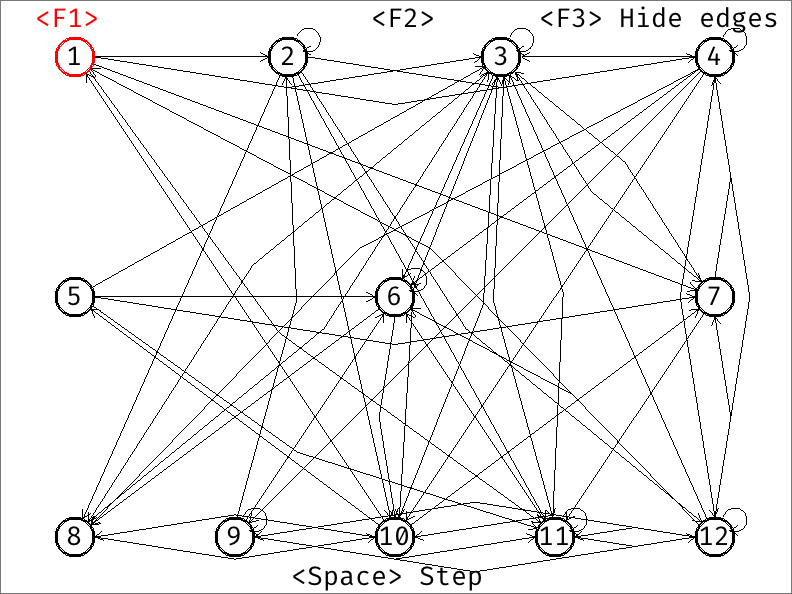
\includegraphics[width=0.5\linewidth]{graph.png}
  \caption{Граф на початку обходу}
\end{figure}
\begin{figure}[ht!]
  \center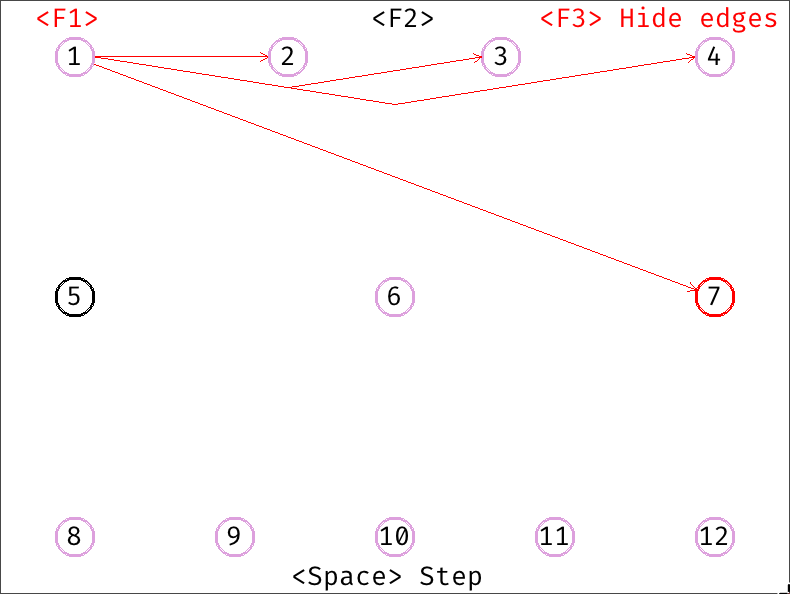
\includegraphics[width=0.5\linewidth]{search.png}
  \caption{Граф на середині обходу (ребра приховані)}
\end{figure}
\begin{figure}[ht!]
  \center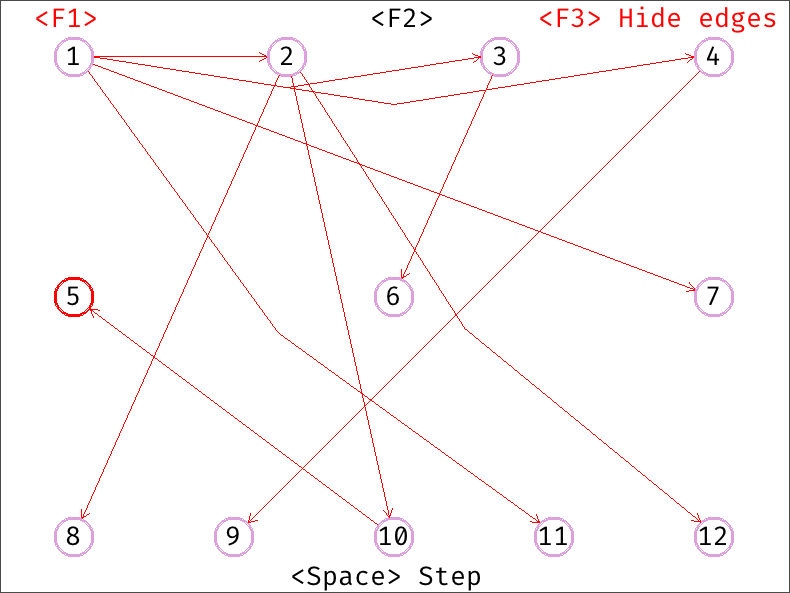
\includegraphics[width=0.5\linewidth]{tree_bfs.png}
  \caption{Дерево обходу BFS}
\end{figure}
\begin{figure}[ht!]
  \center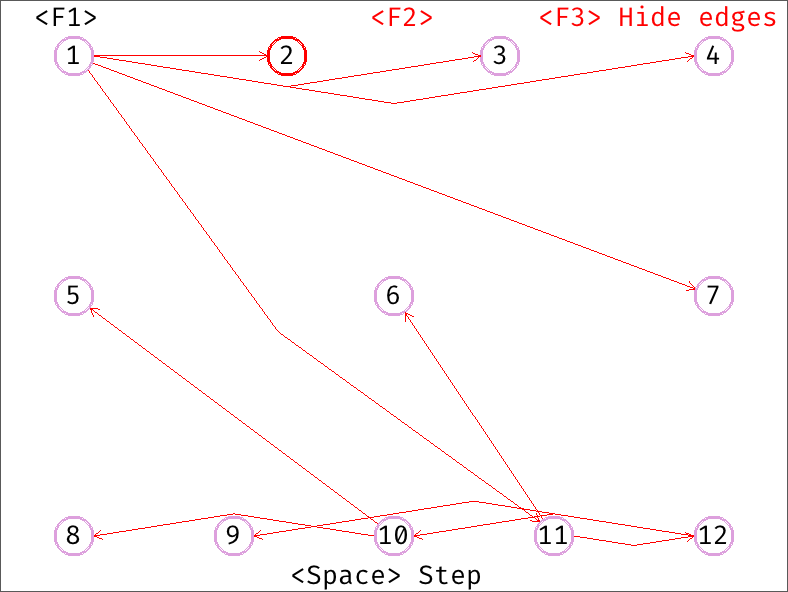
\includegraphics[width=0.5\linewidth]{tree_dfs.png}
  \caption{Дерево обходу DFS}
\end{figure}
\pagebreak

\conclusion%
Імплементував BFS та DFS алгоритми обходу графа, що виконуються покроково.\linebreak
Під час написання коду помітив, що обидва методи відрізняються лише структурою даних для черги,
тому абстрагував крок обходу як операцію над деяким \texttt{SearchStep<Q>}, де \texttt{Q} задає
методи деку \texttt{push} та \texttt{pop}
(для BFS --- з різних кінців списку, для DFS --- з одного).

\end{document}

% vim: ts=2: sw=2
